% ============================================================
%  深圳大学实验报告模板(SZU Experiment Report Template)
% This template can be modified according to the specific requirements of your experiment or project.
% Produced by: Chao Fan and Kewei Ou, AI School of SZU
% ============================================================

\documentclass[a4paper,12pt]{article}

% ----------------------------
% 中文与字体支持
% ----------------------------
\usepackage{fontspec}    % 字体支持
\usepackage{xeCJK}       % 中文字体支持
\setCJKmainfont{Noto Serif CJK SC} % 设置中文字体(Overleaf自带Noto字体)
\usepackage{graphicx}
\usepackage{subcaption}

% ----------------------------
% 页面设置与常用宏包
% ----------------------------
\usepackage{geometry}    % 页面边距控制
\geometry{left=1in, right=1in, top=1in, bottom=1in}

\usepackage{longtable}   % 支持长表格
\usepackage{graphicx}    % 插入图片
\usepackage{fancyhdr}    % 页眉页脚控制
\usepackage{tikz}        % 绘制框线等图形
\usetikzlibrary{calc}    % 坐标计算
\usepackage{verbatim}    % 显示代码块
\usepackage{float}       % 控制图片浮动位置([H]参数)

% ----------------------------
% 页眉页脚设置
% ----------------------------
\pagestyle{fancy}
\fancyhf{} % 清空默认页眉页脚
\fancyhead[L]{深圳大学实验报告} % 左侧页眉文字
\fancyhead[C]{} % 中间空
\fancyhead[R]{} % 右侧空

% ============================================================
%                      文档开始
% ============================================================

\begin{document}

% ============================================================
% 封面页
% ============================================================
\begin{titlepage}
    \centering
    \vspace*{2cm}
    \Huge{\textbf{深 \ 圳 \ 大 \ 学 \ 实 \ 验  \ 报 \ 告}}\\[1.5cm]
    
    \Large{课程名称:\underline{\hspace{2cm}Python程序设计基础\hspace{1.5cm}}}\\[0.5cm]
    \Large{项目名称:\underline{\hspace{2cm}AI图搜图应用开发\hspace{2cm}}}\\[0.5cm]
    \Large{学 \quad \quad 院:\underline{\hspace{2.75cm}人工智能学院\hspace{2.75cm}}}\\[0.5cm]
    \Large{专 \quad \quad 业:\underline{计算机科学与技术(IEEE荣誉班)}}\\[0.5cm]
    \Large{指导教师:\underline{\hspace{4cm}樊超\hspace{4cm}}}\\[0.5cm]
    \Large{报告人:\underline{\hspace{0.5cm}陈泓佳\hspace{0.5cm}} \hspace{0.5cm} 学号:\underline{\hspace{0.5cm}2024104023\hspace{1cm}}}\\[0.5cm]
    \Large{实验时间:\underline{\hspace{2.5cm}2026年1月5日\hspace{2.25cm}}}\\[0.5cm]
    \Large{提交时间:\underline{\hspace{2.25cm}2026年1月16日\hspace{2cm}}}\\[1.5cm]

    \vfill
    \Large{教务处制}
\end{titlepage}

\newpage

% ============================================================
% 正文部分
% ============================================================
\begin{figure}[t]
    \centering
    \includegraphics[width=0.92\linewidth]{figs/基本步骤.png}
    \caption{基本流程}
    \label{fig:vit-arch}
\end{figure}
\section{实验步骤}
本实验较为复杂,所以需要很好的计划才能循序渐进的完成:
\begin{enumerate}
    \item [步骤1]:完成深度学习的部分,填写好dinov2\_numpy.py和preprocess\_image.py的部分并使用老师给的图片和npy文件进行验证。
    \item [步骤2]:下载图片数据库,老师总共给了300w条链接,我将从中提取7692张图片作为我的数据集。并编写了代码将这这些图片转换为特征向量并使用字典存储,\{图片文件名:特征向量\}。除此之外,数据库中还有与图片同名的txt文件用于存储图片的描述。
    \item [步骤3]:编写django框架,并实现一些最最基本的功能,比方说普通的图片识别,以及示例图片的识别。
    \item [步骤4]:增加一些创新的东西,比方说查看历史记录、产出图片张数的选择。
\end{enumerate}
\begin{figure}[t]
    \centering
    \includegraphics[width=0.92\linewidth]{figs/debug文件运行结果.png}
    \caption{修改后的debug文件运行结果}
    \label{fig:vit-arch}
\end{figure}
\section{作业内容结果的描述}
这一部分我将展示非创新内容的结果
\begin{enumerate}
    \item[结果1]:对于深度学习部分,我改写了debug.py,使其可以展示我获取的特征向量与老师的特征向量的差别。采用欧几里得范数(L2 distance)衡量两组特征之间的差异,最终获取差异如下:“猫图像特征差异:0.726,狗图像特征差异:0.546,计算特征向量逐元素的最大绝对误差,结果为 0.088,小于 0.1。”实验结果表明,整体误差控制在合理范围内,不影响特征向量在相似度计算与图像检索任务中的判别能力。因此,本部分通过。
    \item[结果2]:在进行图像内容的下载时,我编写了一段代码download.py去获取这些图片,获取了9332张图片,接着编写了一个程序get\_features.py将这些图像变成特征向量,成功了7692张图片。
    \item[结果3]:关于django部分的内容,在视频中可见,这里不加以赘述。展示的相似图片包含了图片本身以及描述图片的文本。
    
\end{enumerate}

\begin{figure}[t]
    \centering
    \includegraphics[width=0.92\linewidth]{figs/粒子效果展示.png}
    \caption{这张图放大可以看到粒子效果}
    \label{fig:vit-arch}
\end{figure}
\section{创新内容结果的描述}
本处我将展示作业尚未要求但我认为比较创新的部分。
\begin{enumerate}
    \item[创新1]:更加崭新的界面,色调风格借鉴了一个著名的国外网站。本次django的模板,我采用了动态的方式丝滑地向用户展示,使其不会像钢镚一样很突兀。其次,我在进入页面会有粒子效果,由于视频吞画质,可能看不清,对Figure 3放大查看,可以看到有游离的粒子效果,同时我也希望老师可以运行程序看一下,因为确实挺好看的。
    \item[创新2]:我添加了可选展示相似图片的张数,最少5张,最多50张,视频中有展示这一部分。
    \item[创新3]:我添加了用户历史查找记录,每一个用户每一次查找,其图片均会本保存到数据库中,并且其账号与这些图片的url和查找时间绑定,可以实现展示历史记录的功能。
\end{enumerate}

\section{讨论}
本次实验中,我在实践中进一步巩固了numpy的使用技能,不仅掌握了数组操作、线性代数运算和特征向量处理等基础功能,还学会了如何将这些基础操作应用于实际的深度学习特征提取任务中。例如,在实现dinov2图像特征提取的过程中,我通过numpy对图像像素进行预处理、中心裁剪以及特征向量计算,并成功验证了与标准特征的一致性,这大大提升了我对数值计算和高维数据处理的理解能力。

同时,本次实验也加深了我对django框架的理解与使用。我熟悉了从项目创建、路由配置到视图函数编写及模板渲染的完整流程,并能够在框架中集成特征提取模块,实现基本的图像检索系统。这不仅让我掌握了web后端开发的实际操作,也让我理解了前后端协同和数据流转的逻辑,对于构建可部署的应用系统具有直接指导意义。

总体而言,本次实验不仅强化了我在 科学计算和web开发方面的实践能力,也为我在未来开发图像检索、数据分析等应用系统奠定了坚实基础,使我能够更自信地将理论知识应用到实际项目中,并进一步探索人工智能与web技术的结合。本次实验的代码已上传至GitHub:https://github.com/ZSZH12138/Image-search。

\newpage

% ============================================================
% 批阅与成绩评定页
% ============================================================

% 绘制正文外框(包含批阅区域)
\begin{tikzpicture}[remember picture, overlay]
  \draw[thick] 
    ($(current page.north west)+(2cm,-3cm)$) 
    rectangle 
    ($(current page.south east)+(-2cm,2.5cm)$);
\end{tikzpicture}

\vspace{1cm}

% 批阅区
\noindent \textbf{指导教师批阅意见:}
\vspace{5cm}
\hfill

\vspace{1cm}

\noindent \textbf{成绩评定:}
\vspace{2cm}
\hfill

\vspace{1cm}

\noindent \textbf{指导教师签字:}
\vspace{2cm}
\hfill

\vspace{1cm}

% 备注部分
\noindent \textbf{备注:}
\begin{itemize}
    \item 报告内的项目或内容设置,可根据实际情况加以调整和补充。
    \item 教师批改学生实验报告时间应在学生提交实验报告时间后 10 日内。
\end{itemize}

% ============================================================
%                      文档结束
% ============================================================

\end{document}
